% !TEX root = ../thesis-main.tex

\section{Experimental Setup} 
\label{section:4}
Current explanation methods mostly serve individuals with ML expertise~\citep{guidotti-2018-survey,bhatt_explainable_2019}, but they should be extended to cater to users outside of the ML community~\citep{miller-2017-explanations}. 
Unlike previous work, our method, \OurMethod{}, generates contrastive explanations by framing the explanation around the prediction error, and aims to help users understand
\begin{inparaenum}[(i)]
\item what contributed to the large error, and 
\item what would need to change in order to produce a reasonable prediction. 
\end{inparaenum}
Presenting explanations in a contrastive manner helps frame the problem and narrows the user's focus regarding the possible outcomes \citep{hilton-1990-conversational,lipton-1990-contrastive}. 

Our explanations are contrastive because they display to the user what would have needed to change in the input order to obtain an alternative outcome from the model --- in other words, why this prediction results in a large error as opposed to a reasonable prediction. 

\subsection{Dataset and Model}
\label{section:dataset}
Our task is predicting monthly store sales using an internal company dataset with 45 features including financial, workforce and physical store aspects. 
Since not all of our practitioners have experience with ML, using an internal dataset with familiar features allows them to leverage some of their domain expertise. 
The dataset includes 45628 observations from 563 stores, collected at four-week intervals spanning from 2010--2015. 
We split the data by year (training: 2010--2013, test: 2014--2015) to simulate a production environment, and we treat every unique combination of store, interval and year as an independent observation. 
After preprocessing, we have 21415 and 12239 observations in our training and test sets, respectively. 
We train the gradient boosting regressor from scikit-learn with the default settings and obtain an $R^{2}$ of 0.96. 



We verify our assumption that large errors are a result of unusual feature values by generating \OurMethod{} explanations for all instances in our test set using $n$ = 5 features and $m$ = 10000 Monte Carlo simulations. In our dataset, we find that 48\% of instances resulting in large errors have feature values outside the reasonable range for all of the $n$ = 5 most important features, compared to only 24\% of instances resulting in reasonable predictions. 
Although this is not perfect, it is clear that \OurMethod{} produces explanations that are at least somewhat able to distinguish between these two types of predictions. 


%\subsection{Why Existing Solutions are Insufficient}
\subsection{Comparison to LIME}
\label{section:lime}
\citet{hilton-2017-social} states that explanations are selective -- it is not necessary or even useful to state all the possible causes that contributed to an outcome. 
The significant part of an explanation is what distinguishes it from the alternative outcome.
If LIME explanations were suitable for our problem, then we would expect to see different features deemed important for instances resulting in large errors compared to those resulting in acceptable errors. 
This would help the user understand why a particular prediction resulted in a large error. 

However, when generating LIME explanations for our test set using $n$ = 5 features, we do not see much of a distinction in the most important features between predictions that result in large errors and those that do not. 
For example, advertising\_costs is one of the top 5 most important features in 18.8\% of instances with large errors and 18.7\% of instances with reasonable predictions. 
These results are summarized in Table~\ref{table:lime}. 
\medskip

\begin{table}[]
\caption{The top $n=5$ features according to LIME for observations resulting in large errors vs. reasonable predictions.}
\label{table:lime}
\centering
\begin{tabular}{llll}
\toprule
\multicolumn{2}{l}{\textbf{Large errors}} & \multicolumn{2}{l}{\textbf{Reasonable Predictions}} \\
\midrule
advertising\_costs             & 0.188      & advertising\_costs                 & 0.187        \\
total\_contract\_hrs                 & 0.175      & total\_contract\_hrs                    & 0.179        \\
num\_transactions            & 0.151      & num\_transactions               & 0.156        \\
floor\_surface                & 0.124      & total\_headcount                & 0.134        \\
total\_headcount             & 0.123      & floor\_surface                      & 0.122        \\
month                     & 0.109      & month                          & 0.094        \\
mean\_tenure      & 0.046      & mean\_tenure         & 0.046        \\
earnings\_index                & 0.033      & earnings\_index                   & 0.031        \\
\bottomrule
\end{tabular}
\end{table}


%\noindent%
Furthermore, we originally tried to design our control group user study using explanations from LIME, but found that test users from \OurCompany{} could not make sense of the objective questions about prediction errors because LIME does not provide any insight about errors specifically. 
Given that we could not even ask questions about errors using LIME explanations to users without confusing them, it is clear that LIME is inappropriate for our task. 

\subsection{User Study Design}
\label{section:studydesign}
We test our method on a real dataset with real users, both from the retailer. 
We include a short tutorial about predictive modeling along with some questions to check users' understanding as a preliminary component of the study. 
This is because our users are a diverse set of individuals with a wide range of capabilities, including data scientists, human resource strategists, and senior members of the executive team. 
We also include \if0 some\fi participants from \OurUniversity{} to simulate users who could one day work in this environment. 
In total, we have 75 participants: 44 in the treatment group and 31 in the control group. 

All users are first provided with a visual description of the model: a simple scatter plot comparing the predicted and actual sales (as shown in Figure~\ref{fig:pred}). 
We also show a pie chart depicting the proportion of predictions that result in large errors to give users a sense of how frequently these mistakes occur. 
In our case, this is 4\%. 
Since our users are diverse, we want to make our description of the model as accessible as possible while allowing them to form their own opinions about how well the model performs. 
Participants in the treatment group are shown \OurMethod{} explanations, while those in the control group are not given any explanation. 








\begin{figure}[t]
\centering
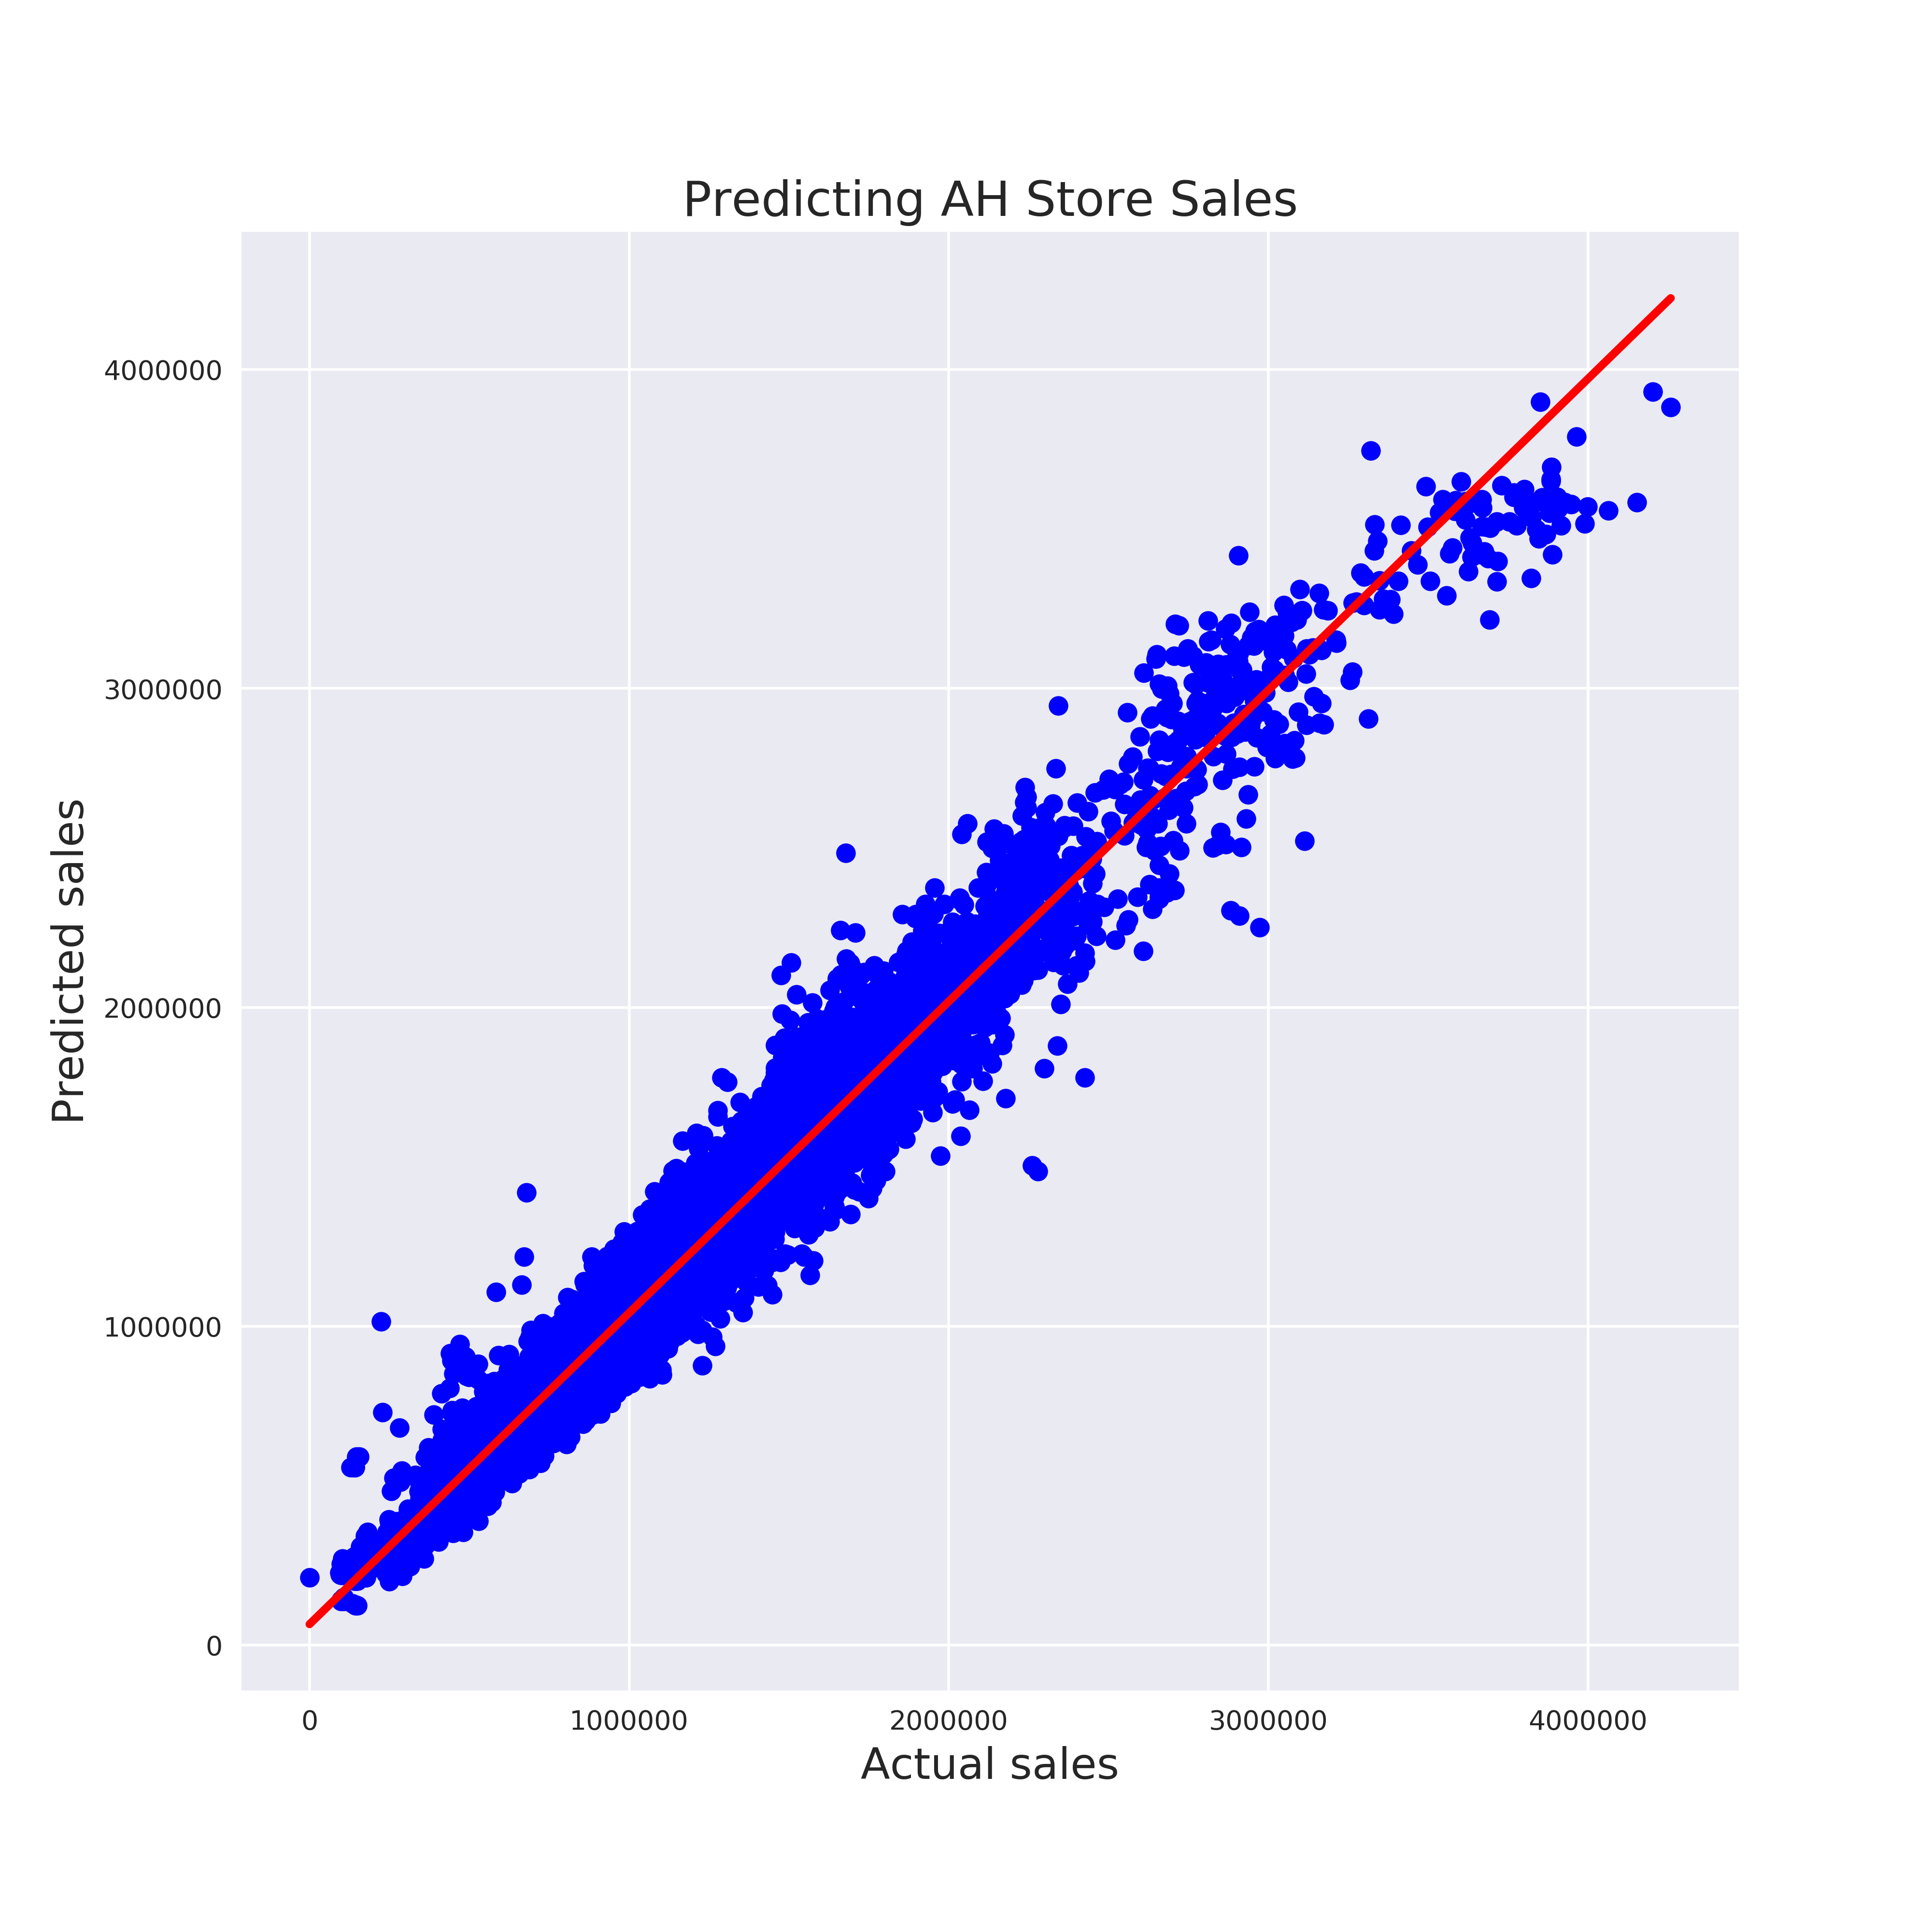
\includegraphics[clip,trim=0mm 0mm 0mm 7.3mm,scale=0.38]{04-research-mcbrp/pred-vs-actual}
\caption{The visual description of the model shown to the users: a graph comparing the predicted sales and actual sales based on the original model. The red line depicts perfect predictions.}
\label{fig:pred}
\vspace*{-.5\baselineskip}
\end{figure}

%\noindent%
The study contains two components, objective and subjective, corresponding to \textbf{RQ3.1} and \textbf{RQ3.2}, respectively. 
The objective component is meant to quantitatively evaluate whether or not users understand explanations generated by \OurMethod{}, while the subjective component assesses the effect of seeing the explanation on users' attitudes towards the model. 
We base the objective component on \textit{human-grounded metrics}, a framework proposed by \citet{doshi-2017-towards}, where the tasks conducted by users are simplified versions of the original task. 
Instead of asking users to correctly predict retail sales values of order $10^6$, we ask them to determine whether or not a prediction will result in a large error. 
%We modify the original sales prediction task into a binary classification one: we ask users to determine whether or not a prediction will result in a large error, as it seems unreasonable to expect humans to correctly predict retail sales values of order $10^6$. 

\begin{table}[h]
\caption{Summary of tasks performed in user study for the treatment and control groups. The subjective questions are asked twice. }
\label{table:study}
\centering
\begin{tabular}{ll}
\toprule
\multicolumn{1}{c}{\textbf{Treatment}} & \multicolumn{1}{c}{\textbf{Control}} \\ 
\midrule
1. Short modeling tutorial        & 1. Short modeling tutorial         \\
2. Visual model description            & 2. Visual model description             \\
3. Subjective questions                & 3. Subjective questions                 \\
4. Objective questions                 & 4. Dummy questions                      \\
5. Subjective questions       & 5. Subjective questions   \\
\bottomrule      
\end{tabular}
\end{table}

\begin{table}[h]
\caption{Summary of simulations performed in objective portion of the user study.}
\label{table:simulations}
\centering
\begin{tabular}{lll}
\toprule
\textbf{Type} & \textbf{Provide user with} & \textbf{User's task} \\ 
\midrule
Forward & (1) Input values & Simulate output  \\
 & (2) Explanation & \\ 
\midrule
Counterfactual & (1) Input values & \multirow[t]{2}{3.4cm}{Manipulate input to change output} \\
 & (2) Explanation  &  \\
 & (3) Output  &  \\ 
\bottomrule
\end{tabular}
\end{table}







To answer \textbf{RQ3.1}, we ask users in the treatment group to perform two types of simulations, both suggested by \citet{doshi-2017-towards} and summarized in Table~\ref{table:simulations}. 
The first is \textit{forward simulation}, where we provide participants with the 
\begin{inparaenum}[(i)]
\item input values, and 
\item explanation. 
\end{inparaenum}
We then ask them to simulate the output --- whether or not this prediction will result in a large error. 
The second is \textit{counterfactual simulation}, where we provide participants with the
\begin{inparaenum}[(i)]
\item input values, 
\item explanation, and 
\item output. 
\end{inparaenum}
We then ask them what they would have needed to change in the input in order to change the output. 
In other words, we want participants to determine how the input features can be changed (according to the trend) in order to produce a reasonable prediction as opposed to one that results in large error. 
These objective questions are designed to test whether or not a participant understands the explanations enough to predict or manipulate the model's output. 
We ask every participant in the treatment group to perform two forward simulations and one counterfactual simulation, and we show the same examples to all users. 

For the control group, we found that we could not ask the objective questions in the same way we did for the treatment group. 
This is because the objective component involves simulating the model based on the explanations (see Table~\ref{table:simulations}), which is not possible if the explanations are not provided. 
In fact, we initially left the objective questions in the control group study, but preliminary testing on some users from \OurCompany{} showed that this was confusing and unclear, similar to when we tried using LIME explanations. 
We were concerned this confusion would skew users' perceptions of the model and therefore convolute the results of \textbf{RQ3.2}. 
Instead, we show participants in the control group the
\noindent
\begin{inparaenum}[(i)]
\item input values, and 
\item output -- whether or not the example resulted in a large error. 
\end{inparaenum}
In this case, we ask them \emph{if they have enough information} to determine why the example does (or does not) result in a large error. 
This serves as a dummy question to engage users with the task without confusing them. 
We cannot ask users in the control group to simulate the model since they do not see the explanations, but we want to mimic the conditions of the treatment group as closely as possible. 
Therefore, \textbf{RQ3.1}, is solely evaluated on users from the treatment group. 

To answer \textbf{RQ3.2}, we contrast results from the treatment and control groups. 
We ask both groups of users the same four subjective questions twice, once towards the beginning of the study and once again at the end. 
We ask the questions at the beginning of the study to evaluate the distribution of preliminary attitudes towards the model, based solely on the visual description. 
We ask the questions at the end of the study to evaluate the effectiveness of \OurMethod{} explanations, by comparing the results from the treatment and control groups. 
The questions we devised are based on the user study by \citet{terhoeve-2017-news}. 
Table~\ref{table:study} summarizes the experimental setup for the treatment and control groups. 
Again, the treatment and control groups are treated exactly the same with the exception of the objective questions -- we only ask these to the treatment group since we cannot ask users to simulate the model without giving them the explanation. 